%!TEX root = ./main.tex

\section{The model}

\begin{frame}{The model}

\alert{Goal}: given a set of $n$ data with $p$ variables, simultaneously infer the conditional dependence structure of such variables and their clustering.

\pause

\alert{Constraint}: the partition must respect the original order of the variables.
\pause
\begin{align*}
    \bm{y}_1, \ldots, \bm{y}_n \mid \bm{K} & \iid \mathcal{N}_p(\mathbf{0}, \bm{K}^{-1} ) \\
    \bm{K} \mid G & \sim \GWish(b, D)\\
    P((i,j)&\in E\mid \bm{z},Q) = Q_{z_{i} z_{j}},\,\text{independent}\\
        Q_{rs} \mid \bm{z} &\ind \Beta(\alpha,\beta), 1\leq r\leq s\leq M\\
    \rho & \sim f_{\rho} \left(\rho\right)
\end{align*}

Notation for the partition: $\rho$ vector of cardinalities, $\bm{z}$ vector of groups memberships.

The prior for the \alert{partition} $f_{\rho}(\rho)$ is (5) from \cite{martinezNonparametricChangePoint2014}.

\end{frame}

\begin{frame}

$Q$ is marginalized out.
\pause

The prior for the \alert{graph} given the vector of group memberships is
\[
    P(G\mid \bm{z})
    =
    \prod_{u=1}^{M}\prod_{v=u}^{M}
    \frac{B(\alpha + S_{uv}, \beta+ S^{\star}_{uv})}{B(\alpha,\beta)}
\]
where 
\begin{itemize}
    \item $S_{uv}$ is the sum of the edges between group $u$ and $v$.
    \item $S^{\star}_{uv}$ is the sum of the ``non-edges'', namely $S^{\star}_{uv} = T_{uv} - S_{uv}$ and $T_{uv}$ is the total number of possible edges.
\end{itemize}


\end{frame}




\begin{frame}{Main references}
    % GGM
    \nocite{colombiLearningBlockStructured2022a}
    \nocite{mohammadiBayesianStructureLearning2015a}
    % SBM
    \nocite{legramantiExtendedStochasticBlock2022}
    % Changepoint
    \nocite{bensonAdaptiveMCMCMultiple2018}
    \nocite{martinezNonparametricChangePoint2014}
    
    \printbibliography
    \renewcommand*{\bibfont}{\small}
\end{frame}

\begin{frame}[plain]
    % Add background to content page
    \AddToShipoutPictureFG*{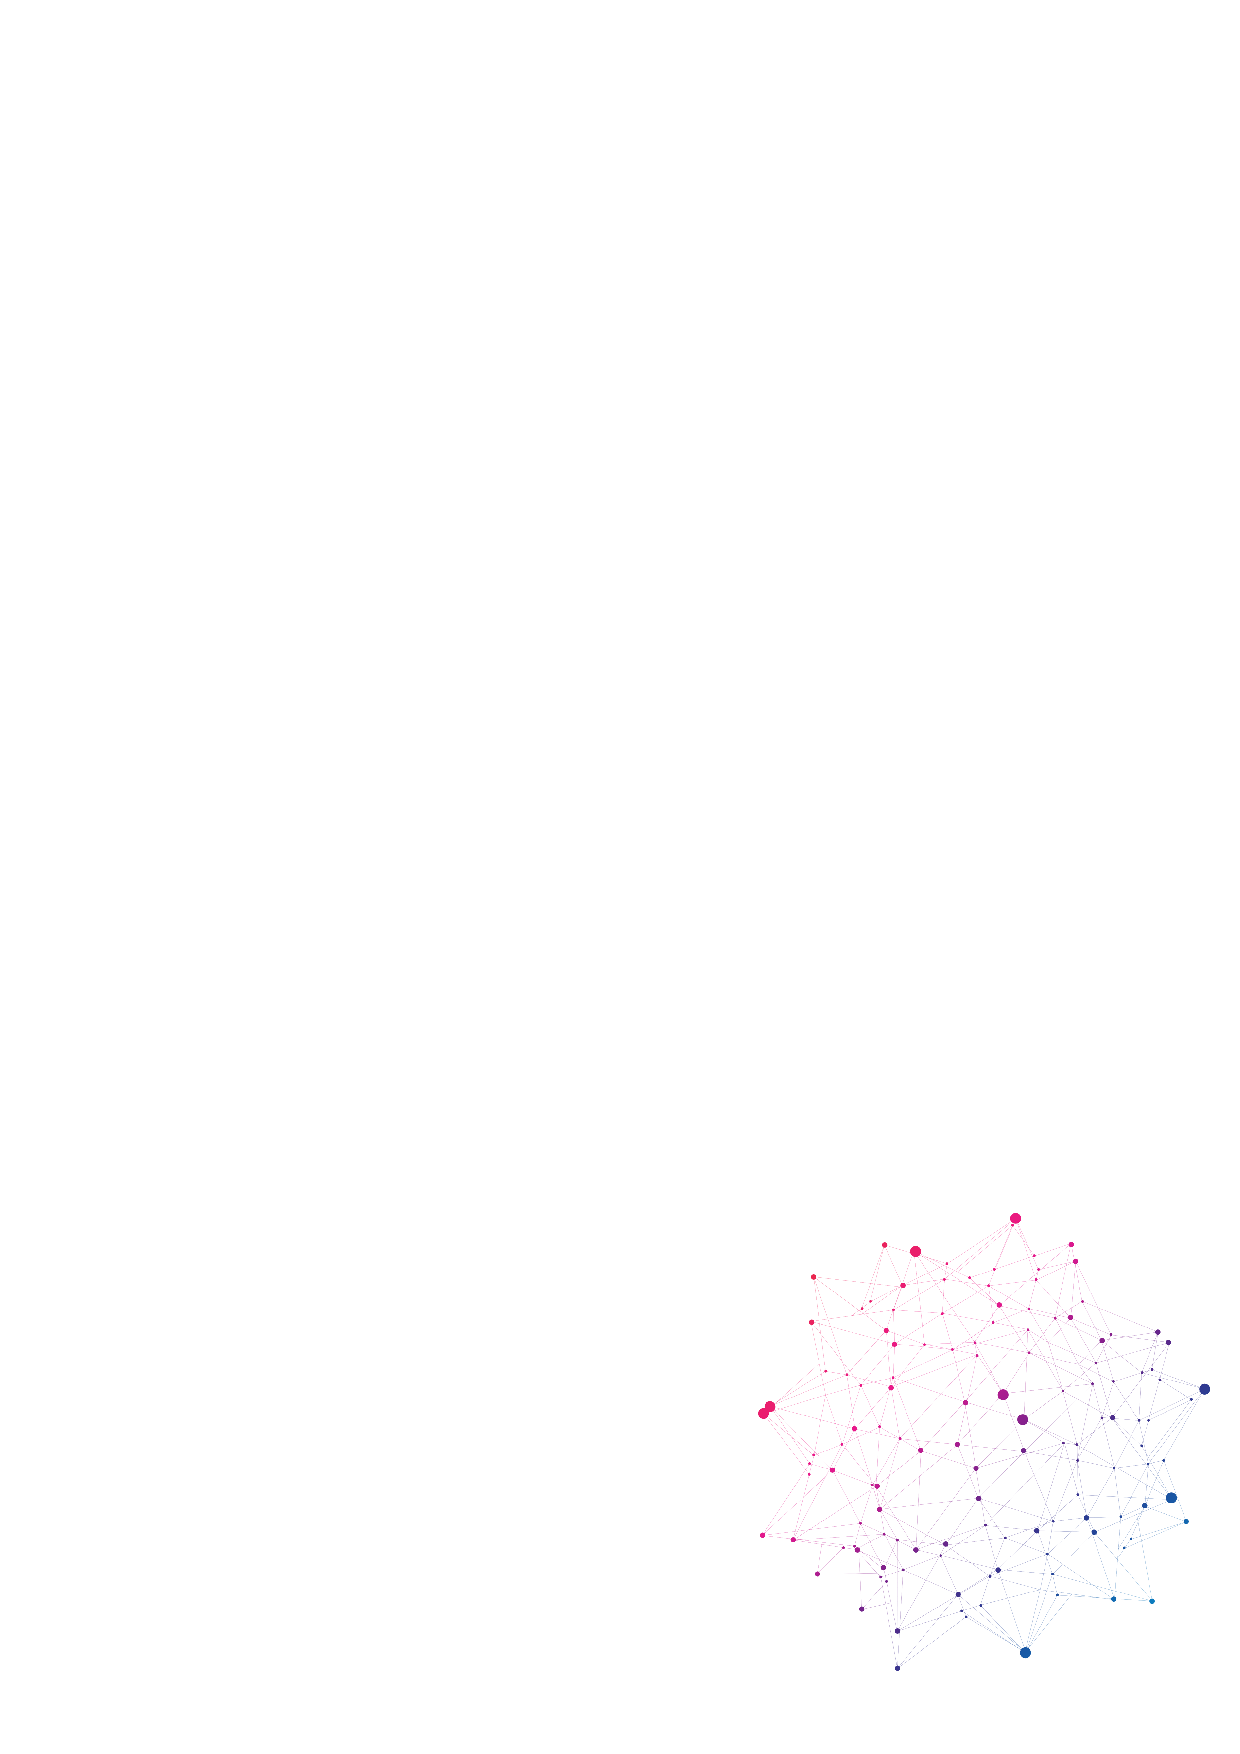
\includegraphics[width=\paperwidth]{Images/background.pdf}}
    \vspace*{1.2cm}
    \hspace*{1cm}{\Large Thank you!}\\
    \vspace*{0.6cm}
    \hspace*{1cm}{\Huge \alert{Any questions?}}
\end{frame}
